	\documentclass[border = 12]{standalone}
	\usepackage{amsmath}
	\usepackage{stix}
	\usepackage{tikz}
	\usepackage{tkz-euclide}
	\usepackage{makecell}
	\usepackage{ifthen}
	\usepackage{pgfmath}
	\definecolor{blue}{RGB}{0,51,255} 
	\usetkzobj{all}
	
	\usetikzlibrary{intersections}
	\usetikzlibrary{decorations.markings}
	\usetikzlibrary{angles}
	\usetikzlibrary{quotes}
	\usetikzlibrary{calc}
	\usetikzlibrary{arrows}
	\usetikzlibrary{arrows.meta}
	\usetikzlibrary{shapes.geometric}
	\usetikzlibrary{patterns}
	\usetikzlibrary{shapes}
%
\definecolor{Grey}{RGB}{76,76,78}
\definecolor{Blue}{RGB}{85,164,224}
\definecolor{Red}{RGB}{225,75,59}
\definecolor{Green}{RGB}{16,158,36}
\definecolor{Orange}{RGB}{243,162,3}
\definecolor{Purple}{RGB}{124,36,231}
\definecolor{Fushia}{RGB}{225,50,162}



%
\definecolor{Grey1}{RGB}{130,130,131}
\definecolor{Blue1}{RGB}{98,170,223}
\definecolor{Red1}{RGB}{236,98,88}
\definecolor{Green1}{RGB}{105,186,108}
\definecolor{Orange1}{RGB}{251,192,79}
\definecolor{Purple1}{RGB}{160,114,235}
\definecolor{Fushia1}{RGB}{237,97,174}

\usepackage{tikz-3dplot}
\usepackage{tikz}
\usetikzlibrary{calc,intersections,arrows.meta}
\begin{document}
	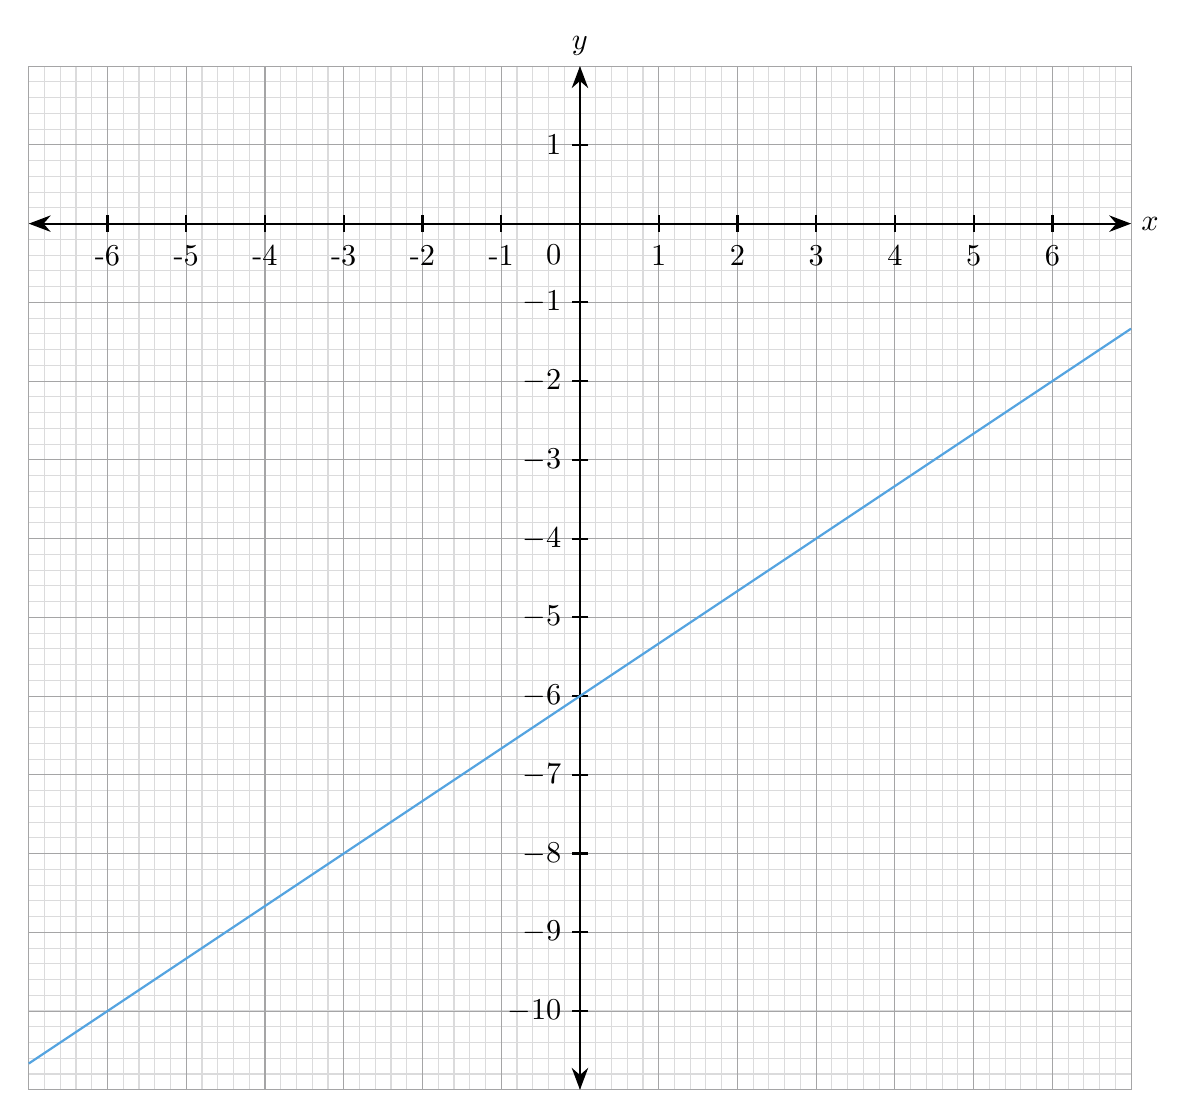
\begin{tikzpicture}
	
	\begin{scope}[>={Stealth[scale=1.2]}, thick,font=\fontsize{11.25}{11.25}\selectfont]
	
	\pgfgettransformentries{\mya}{\myb}{\myc}{\myd}{\mys}{\myt}
	\pgfmathsetmacro{\preserve}{1/\mya}
	
	\draw [thin,Grey!20,step=0.2]  (-7,-11) grid (7,2);
\draw [thin,Grey!50,step=1]  (-7,-11) grid (7,2);
	
	
	\foreach \x/\m in {-6,...,-2,-1,1,2,...,6}
	\draw (\x,3pt*\preserve) -- (\x,-3pt*\preserve)
	node at (\x,0) [below=0.15] {\nagwaMathLabel{\m}};
	
	
	\foreach \y/\n in {-10,...,-2,-1,1}{
		\draw (3pt,\y)--(-3pt,\y) node [left] {$\n$};}
	
	\foreach \x/\m in {0}
	\node at (\x,0) [below left=4pt and 3pt] {\nagwaMathLabel{\m}};	
	\draw [<->] (7,0) node[anchor=west] {$x$} --(-7,0);
	
	\draw [<->] (0,-11)--(0,2)node[anchor=south]{$y$};	

		
		\draw [ thick,Blue,samples=100,domain=-7:7] plot (\x,{((2*\x)-18)/3});
		
		\end{scope}
		\end{tikzpicture}
	\end{document}
